\chapter{barra superior}
\begin{center}
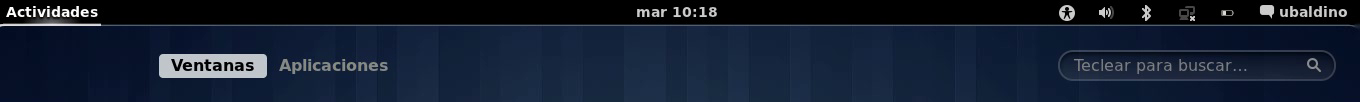
\includegraphics[scale=0.45]{img/barra2.png} 
\end{center}
GNOME 3 cuenta con una interfaz de usuario completamente reinventada, diseñada para permanecer fuera de su vista, minimizar las distracciones, y ayudarle a trabajar. La primera vez que inicie una sesión, verá un escritorio vacío y la barra superior.\\

La barra superior permite el acceso a las ventanas y aplicaciones, su calendario y citas, y las propiedades del sistema como el sonido, la red, y la energía. Bajo su nombre en la barra superior, puede establecer su disponibilidad, cambiar su perfil o configuración, salir o cambiar de usuario, o apagar el equipo.
\section{Vista de actividades}
Para acceder a sus ventanas y aplicaciones, pulse el botón Actividades, o simplemente lleve el puntero del ratón a la esquina activa. También puede pulsar la tecla Windows en su teclado. Puede ver sus ventanas y aplicaciones en la vista. También puede empezar a escribir para buscar aplicaciones, archivos o carpetas.\\

A la izquierda de la vista, encontrará el tablero. El tablero le muestra sus aplicaciones favoritas y en ejecución. Pulse en cualquier icono en el tablero para abrir dicha aplicación. Si la aplicación se está ejecutando, pulsar en el icono abrirá la ventana utilizada ​​más recientemente.\\
Para seleccionar una ventana en una aplicación en ejecución, o para abrir una ventana nueva, pulse con el botón derecho del ratón sobre la aplicación. También puede arrastrar el icono sobre la vista general, o sobre cualquier miniatura de área de trabajo a la derecha.
Cuando entre en la vista, inicialmente estará en la vista de las ventanas. Esto muestra las miniaturas de todas las ventanas en el área de trabajo actual. Pulse en cualquier ventana para dar el foco la ventana y salir de la vista. También puede usar la rueda de desplazamiento del ratón para aumentar cualquier miniatura de la ventana.\\
Pulse en Aplicaciones para entrar en la vista de aplicaciones. Esto le muestra todas las aplicaciones instaladas en su equipo. Pulse en cualquier aplicación para ejecutarla, o arrastre una aplicación a la vista o sobre la miniatura del espacio de trabajo. También puede arrastrar una aplicación al tablero para que sea uno de los favoritos. Sus aplicaciones favoritas permanecerán en el tablero, incluso cuando no estén en funcionamiento, para que pueda acceder a ellas rápidamente.
\section{Reloj, calendario y citas}
\begin{center}
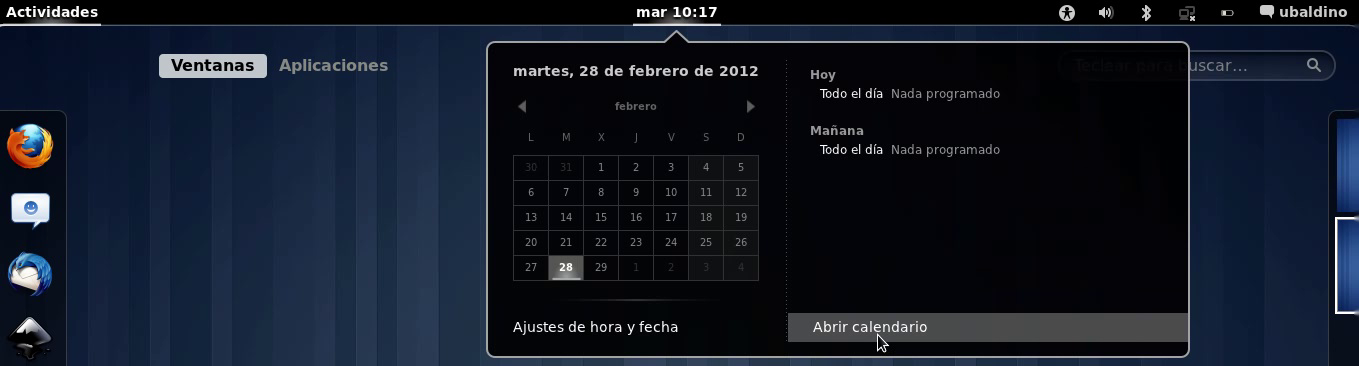
\includegraphics[scale=0.5]{img/calendario.png} 
\end{center}
Pulse en el reloj en el centro de la barra superior para ver la fecha actual, un calendario mensual y una lista de sus próximas citas. También puede acceder a la configuración de fecha y hora y abrir totalmente su calendario de Evolution directamente desde el menú.
\subsection{Citas de calendario}
Esto requiere que Evolution esté instalado en su equipo.\\
La mayoría de las distribuciones tienen instalado Evolution de forma predeterminada. Si la suya no lo tiene, puede querer instalarlo usando el gestor de paquetes de su distribución.\\

{\bf Para ver sus citas:}
\begin{enumerate}
\item Pulse en el reloj en la barra superior.
\item Seleccione en el Calendario la fecha para la que quiere ver sus citas.
\item El calendario mostrará las citas existentes a la derecha. Ya que las citas se añaden en Evolution, éstas aparecerán en la lista de citas del reloj.\\
%%%imagen

Para conseguir rápidamente le calendario completo de Evolution, pulse en el reloj y pulse Abrir calendario.\\
Esto funcionará solo si tiene una cuenta de Evolution. En caso contrario, aparecerá una ventana con los pasos necesarios para añadir su primera cuenta.
\end{enumerate}
\section{Usted y su equipo}
\begin{center}
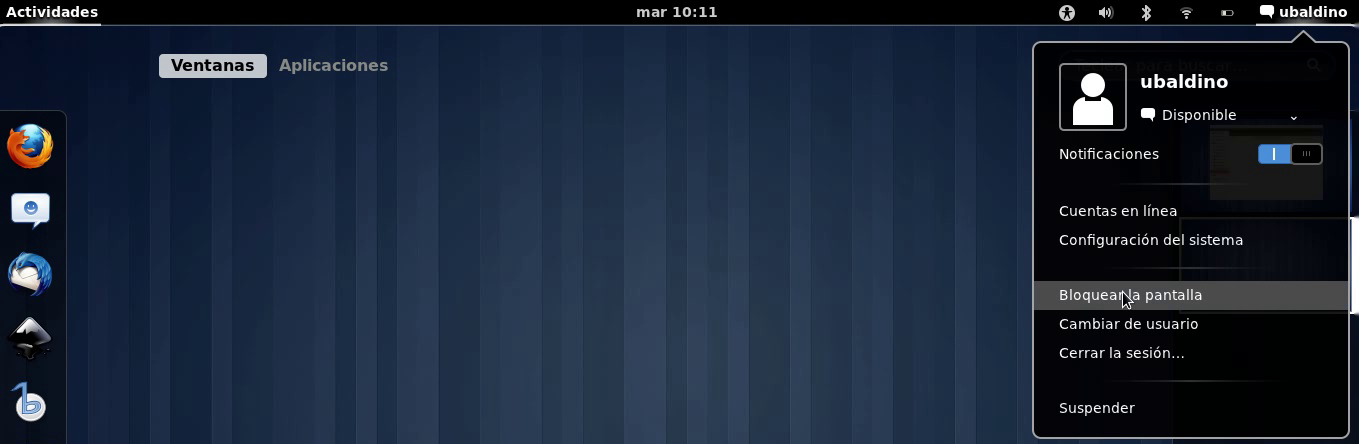
\includegraphics[scale=0.45]{img/usuario.png} 
\end{center}
Pulse en su nombre de usuario en la esquina superior derecha de la pantalla para gestionar su perfil y su equipo.\\
Puede establecer rápidamente su disponibilidad directamente desde el menú. Cuando usa la aplicación de mensajería instantánea Empathy, esto establecerá su estado para que sus contactos lo vean.\\

El menú también le permite editar su información personal y cambiar la configuración del sistema.\\

Al dejar su equipo, puede bloquear la pantalla para evitar que otras personas lo usen. Puede rápidamente cambiar de usuario sin necesidad de iniciar la sesión completamente para dar a alguien acceso al equipo. O bien, puede suspender o apagar el equipo desde el menú.
%%%%%imagen
\subsection{Cerrar la sesión, apagar o cambiar de usuario}
Cuando haya terminado de usar su equipo, puede apagarlo, suspenderlo (para ahorrar energía), o dejarlo encendido y cerrar la sesión.
\subsubsection{Cerrar la sesión o cambiar de usuario}
Para permitir que otros usuarios usen su equipo, puede salir de la sesión, o seguir conectado y simplemente cambiar de usuario. Si cambia de usuario, todas las aplicaciones seguirán funcionando y todo estará donde lo dejó cuando vuelva a iniciar sesión.\\
Para Salir de la sesión o Cambiar de usuario, pulse sobre su nombre en la barra superior y seleccione la opción apropiada.
\subsubsection{Bloquear la pantalla}
Si deja su equipo durante un breve periodo de tiempo, debe bloquear la pantalla para evitar que otras personas tengan acceso a sus archivos y ejecuten aplicaciones. Cuando vuelva, simplemente introduzca su contraseña para volver a iniciar la sesión. Si no bloquea la pantalla, se bloqueará automáticamente tras un cierto tiempo.\\

Para bloquear la pantalla, pulse sobre su nombre en la barra superior y seleccione Bloquear la pantalla.\\

Cuando su pantalla está bloqueada otros usuarios pueden iniciar sesión en sus propias cuentas pulsando Cambiar de usuario en la pantalla de contraseña. Puede volver a su escritorio cuando hayan terminado.
\subsubsection{Suspender}
Para ahorrar energía, suspenda su equipo cuando no lo esté usando. Si usa un equipo portátil, GNOME suspende su equipo automáticamente cuando cierra su tapa. Esto guarda su estado en la memoria de su equipo y apaga la mayor parte de las funciones de su equipo. Durante la suspensión se sigue usando una cantidad muy pequeña de energía.\\

Para suspender su equipo manualmente, pulse sobre su nombre en la barra superior y seleccione Suspender.
\subsubsection{Apagar o reiniciar}
Si quiere apagar su equipo por completo o hacer un reinicio total, primero cierre la sesión pulsando en su nombre en la barra superior y seleccionando Cerrar sesión. Volverá a la pantalla de inicio de sesión. En esta pantalla, pulse el icono de encendido en la barra superior y seleccione Reiniciar o Apagar.\\
Si hay otros usuarios conectados, no podrá apagar o reiniciar el equipo, porque esto cerraría sus sesiones. Si es un usuario administrativo, se le pedirá su contraseña para apagar.\\

Si necesita apagar o reiniciar rápidamente lo puede hacer sin cerrar la sesión. Pulse en su nombre, en la barra superior y mantenga pulsada la tecla Alt. La opción Suspender cambiará a Apagar. Seleccione apagar o reiniciar.
\section{Bandeja de mensajes}
\begin{center}
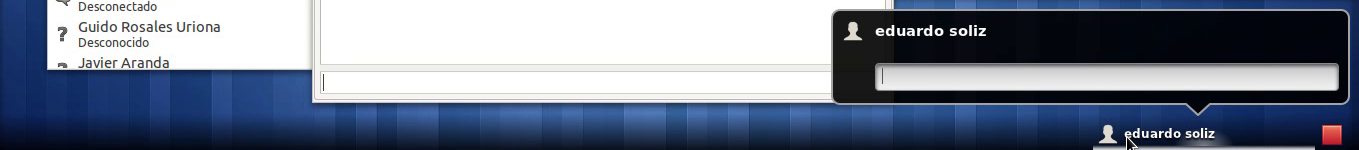
\includegraphics[scale=0.5]{img/bandeja.png} 
\end{center}
La bandeja de mensajes puede mostrarse moviendo el ratón a la esquina inferior derecha. Aquí es donde se almacenan las notificaciones hasta que esté listo para verlas.
\subsection{¿Qué es una notificación?}
Si una aplicación o un componente del sistema quiere llamar su atención, mostrará una notificación en la parte inferior de la pantalla.\\
Por ejemplo, si recibe un nuevo mensaje de chat, hay nuevas actualizaciones disponibles para su equipo o la batería está baja, recibirá una notificación informándole de ello.\\

La notificación aparecerá primero como una sola línea, de modo que no le distraiga. Puede mover el ratón sobre ella si quiere ver su contenido completo.

\subsection{Ocultar notificaciones}
Si está trabajando en algo y no quiere que le molesten, puede desactivar las notificaciones. Simplemente pulse en su nombre en la barra superior y seleccione Notificaciones para cambiarlo a Apagado.\\
Cuando esté apagado, la mayoría de las notificaciones no se mostrarán como mensajes emergentes en la parte inferior de la pantalla. Las notificaciones importantes, tales como batería críticamente baja, se seguirán mostrando. Las notificaciones seguirán estando disponibles en la bandeja de mensajería al mover el ratón a la esquina inferior derecha, y se mostrarán cuando seleccione estar disponible de nuevo.